\documentclass[a4paper,11pt]{article}

\usepackage[spanish]{babel}
\usepackage[utf8]{inputenc}
\usepackage{hyperref}
\usepackage{amssymb}
\usepackage{graphicx}
\usepackage{amsmath}
\graphicspath{{images/}} 

\author{Daniel Monjas Miguélez}
\title{FR: Tema 4}

\begin{document}
\begin{titlepage}
\centering
    \vfill
    {\bfseries\Large
        Fundamentos de Bases de Datos: Tema 4\\
        28 de Noviembre del 2020\\
        A year to Forget \\
        \vskip2cm
        Daniel Monjas Miguélez\\
    }    
    \vfill
    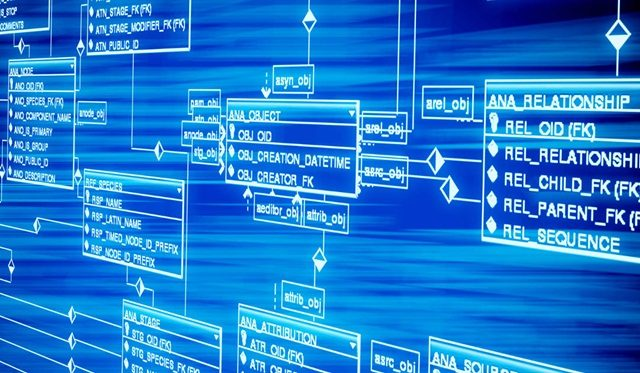
\includegraphics[width=13cm]{bases_datos.jpg}
    \vfill
    \vfill
\end{titlepage}

\newpage
\tableofcontents
\newpage

\section{Introducción}

Una base de datos sirve para almacenar de forma permanente grandes cantidades de datos con el propósito principal de gestionar de forma eficiente los datos y su almacenamiento. Esto tiene sus consecuencias tanto en la organización lógica de los datos, como en su organización física. \\

\textbf{Nivel interno}:
\begin{itemize}
\item Expresa en última instancia, las operaciones sobre los datos (creación, alteración y recuperación) en términos de actuación sobre unidades mínimas de almacenamiento denominadas páginas o bloques de base de datos.

\item Provee al administrador de mecanismos para optimizar el almacenamiento y el acceso a los datos.

\item Se encuentra implementado en el SGBD.
\end{itemize}

\textbf{Nivel físico:}
\begin{itemize}
\item Se encuentra implementado en el SO.

\item Proporciona al SGBD una capa de abstracción sobre el hardware.

\item Realiza el acceso a los medios de almacenamiento mediante llamadas a los servicios de archivos proporcionados por el SO.
\end{itemize}

\textbf{Jerarquía de memoria}

\begin{figure}[h]
\centering
\caption{Jerarquía de memoria}
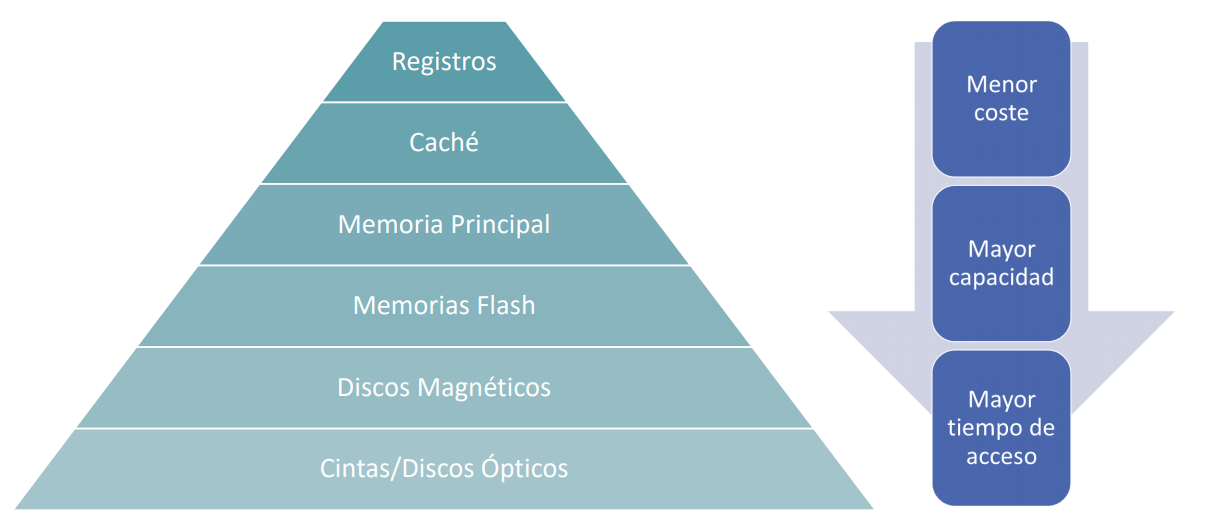
\includegraphics[scale=1,width=1\textwidth]{jerarquia_memoria.png}
\end{figure}

\textbf{Memoria principal}

Es el dispositivo de almacenamiento primario de los ordenadores. Esta hace trabajos de caché de la porción de la BD de uso más reciente, y es  el elemento intermedio que ubica de forma temporal los datos afectados por las operaciones. \\

El nivel interno debe optimizar el uso de la memoria principal, pues esta es rápida lo que significa que acelera el procesamiento y además es cara, luego se debe optimizar su uso. \\

La memoria principal es volátil, es decir, se pierde cuando se apaga el sistema (o se cae). El nivel interno debe garantizar que la información contenida tenga un respaldo en almacenamiento secundario para que esta no se pierda. \\

Para acelerar el acceso a los datos se utilizan distintos niveles de caché. \\

\textbf{Discos duros}

Se trata del dispositivo de almacenamiento más utilizado en BD. Estos se componene de un conjunto de discos magnético con dos caras, donde cada cara tiene un conjunto de pistas concéntricas (cilindro:la misma pista de todas las caras). Cada una de estas pistas se divide en sectores (512 Bytes) con la misma capacidad de almacenamiento (bloque). Luego para localizar un bloque se busca en que cilindro está, luego se va al correspondiente disco magnético y se busca el sector. \\

En los discos duros se tienen en cuenta los siguientes parámetros:

\begin{itemize}
\item Capacidad
\item Tiempo medio de acceso
\item RPM
\item Velocidad sostenida de lectura/escritura
\end{itemize}

Ahora se verán unas medidas de rendimiento:

\begin{itemize}
\item Tiempo medio de acceso ($t_a$): tiempo medio transcurrido entre una instrucción y la obtención de la información. 

\item Tiempo medio de búsqueda ($t_b$): tiempo medio de posicionamiento en pista.

\item Tiempo de latencia rotacional ($t_l$): tiempo medio de procesamiento en sector

\item Tiempo medio entre fallos (MTBF)
\end{itemize}

\begin{equation*}
t_a=t_b+t_l
\end{equation*}

\begin{figure}[h]
\centering
\caption{Ejemplo Disco Duro}
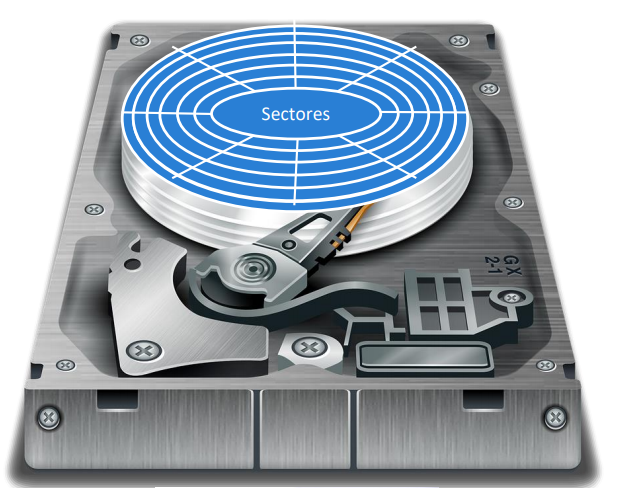
\includegraphics[scale=1,width=0.8\textwidth]{disco_duro.png}
\end{figure}

\section{Método de acceso a la BD}

\begin{figure}[h]
\centering
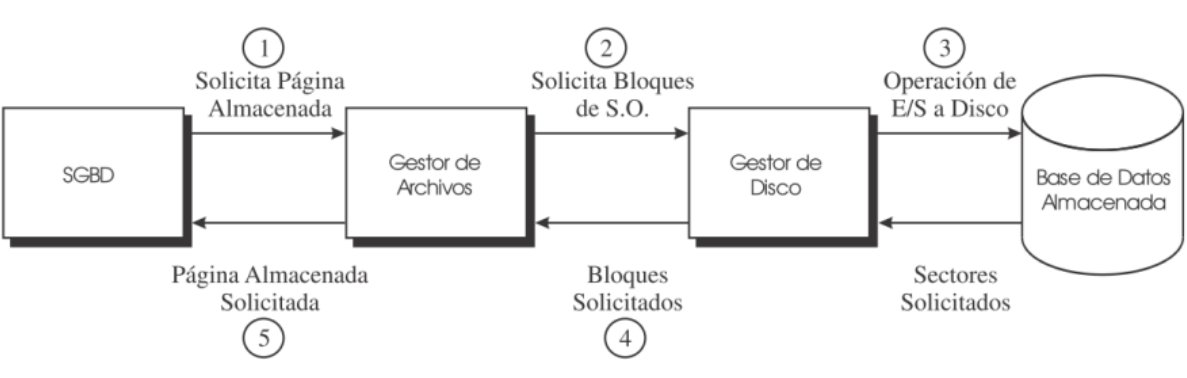
\includegraphics[scale=1,width=1.0\textwidth]{transformacion.png}
\end{figure}

Para que el gestor de almacenamiento pueda localizar un registro almacenado, se utiliza el RID(Record IDentifier), el cual se compone de una página y su correspondiente offset dentro de la misma. \\

Cada registro almacenado tiene una cabecera que contiene el número y tipo de columnas que lo integran así como los datos, que se corresponde con el contenido de las columnas. \\

Las páginas o bloque de la BD deben tener un tamaño múltiplo de las páginas del SO (mínima unidad de E/S). \\

Para recuperar un registro almacenado hay que determinar la página de BD que lo contiene y entonces recuperar los bloque de disco que la integran. \\

Hay que organizar la estructura de almacenamiento y los métodos de acceso, de forma que se optimice la interacción con los dispositivos de almacenamiento secundario. \\

\textbf{\underline{Deben minimizarse las operaciones E/S al almacenamiento secundario}} \\

\begin{figure}
\centering
\caption{Ejemplo RID}
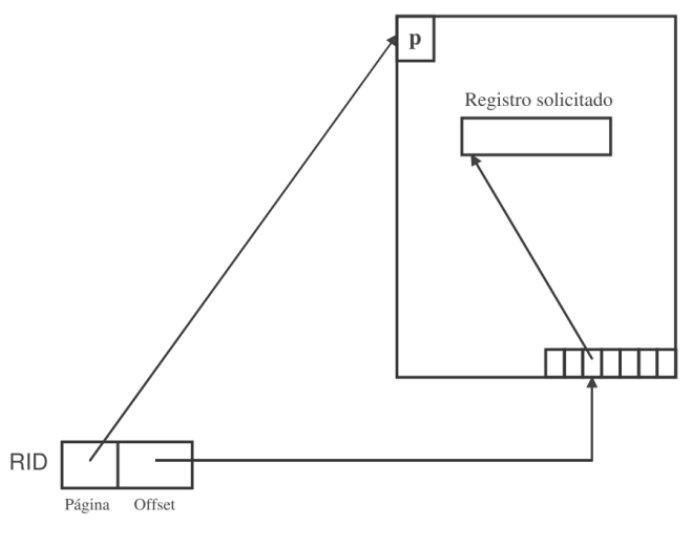
\includegraphics[scale=1,width=0.8\textwidth]{rid.png}
\end{figure}

\textbf{El Gestor de Disco del SO}

Normalmente el SGBD interactúa con la BD almacenada en el sistema de almacenamiento secundario a través del gestor de disco del SO. \\

El gestor de disco organiza los datos en conjuntos de bloques o archivos de SO. Una BD puede utilizar uno o varios de estos archivos para almacenar su contenido. \\

También se encarga de gestionar el espacio libre en el disco. \\

Como funciones elementales de un Gestor de Disco del SO tenemos:

\begin{itemize}
\item Crear un nuevo archivo de SO
\item Eliminar un archivo de SO existente
\item Añadir un bloque nuevo al conjunto de bloques c
\item Eliminar el bloque b del conjunto de bloques c
\item Devolver el bloque b del conjunto de bloques c
\item Reemplazar el bloque b dentro del conjunto de bloques c
\end{itemize}

\textbf{El Gestor de Archivos del SGBD}

Se trata de un componente del SGBD que se encarga de hacer la transformación entre campos, registros y archivos almacenados y bloques y conjuntos de bloques (que pueda entender el gestor de disco), así como de organizar los datos de manera que se minimice el tiempo de recuperación, es decir, minimizando las E/S a disco. \\

Entre las funciones básicas del Gestor de Archivos del SGBD tenemos:

\begin{itemize}
\item Crear un nuevo archivo almacenado. Para ello asocia al archivo un conjunto de páginas o bloques de la BD.

\item Eliminar un archivo almacenado

\item Recuperar el registro almacenado r del archivo almacenado a. Normalente, el SGBD proporciona el RID. Sólo hay que obtener en memoria la página que contiene el registro para extraerlo.

\item Añadir un nuevo registro almacenado al archivo almacenado a. Hay que localizar la página de BD más apropiada de las pertenecientes al archivo almacenado. Si no se puediera, se solicita una nueva página. Por último se devuelve al SGBD el RID.

\item Eliminar el registro r del archivo almacenado a. Hay que recuperar la página de BD que contiene dicho registro y marcar el espacio ocupado por el registro en dicha página como disponible.

\item Actualizar el registro r en el archivo almacenado a. Recupera la página de la BD que contiene el registro que se desea actualizar. Trata de sustituir la información. Si no se puede, se intenta ubicar en otra página.
\end{itemize}

\section{Representación de la BD en el nivel interno}

La BD se representa de diferentes forma en los diferentes niveles de la arquitectura del SGBD. Su representación en el nivel interno no tiene por qué coincidir con su representación en el nivel conceptual. Cada conjunto de registros del mismo tipo no tiene por qué ser un fichero. \\

El nivel interno debe traducir las estructuras del nivel conceptual a otras estructuras intermedias más cercanas al almacenamiento real de los datos (nivel físico). \\

\textbf{Agrupamiento:}

\begin{itemize}
\item La BD en el nivel interno: Conjunto de páginas en las que se van ubicando los registros. 

\item Agrupamiento Intra-Archivo. Ubicar en una misma página registros del mismo tipo. Es el más frecuente.

\item Agrupamiento Inter-Archivo. Ubicar en una página registros de distinto tipo. Ha de existir relación (por ejemplo entidades fuerte-débil).
\end{itemize}

No existe una relación directa fichero-almacenado/fichero-físico, ya que todos los conjuntos de páginas se irán almacenando, con toda probabilidad, en uno o varios ficheros físicos.

\section{Organización y Métodos de Acceso}
El objetivo es minimizar el número de accesos a disco, luego se deben minimizar la cantidad de páginas de BD involucradas en una operación BD. \\

De las organizaciones vistas anteriormente, ninguna es mejor en términos absolutos. Para medir la 'calidad' de una organización se utilizan los siguientes criterios básicos:

\begin{itemize}
\item Tiempo de acceso a los datos requeridos
\item Porcentaje de memoria ocupada por los datos requeridos con respecto a las páginas de BD que los contienen.
\end{itemize}

Trabajaremos a dos niveles, organización de registros de datos a nivel de almacenamiento y adición de estructuras complementarias para acelerar el acceso a dichos registros.

\section{Organización Secuencial}
Se dice fichero de acceso secuencial a aquellos en los que los registros están almacenados consecutivamente. Para acceder a un registro determinado debemos pasar obligatoriamente por los registros que le preceden. Los registros suelen estar ordenador por una clave (clave física). \\

Un ejemplo sería, mostrar la relación completa de departamentos. Esta consulta se resuelve rápidamente si los departamentos están almacenados conjuntamente en bloques contiguos de un fichero.\\

Sin embargo, si queremos plantear consultas por valor de clave o por rango de valores: \\

El primer caso implica recorrer uno tras otro cada uno de los registros, y en el peor de los casos (no encotrar dicho departamento en la lista) supone recorrer de forma completa el fichero. Búsqueda con complejidad O(n). \\

En el segundo caso se realiza la búsqueda por valor de clave de la cota inferior del intervalor. Se continúa hasta alcanzar la cota superior. Si están ordenador por el valor de la clave.

\begin{figure}[h]
\centering
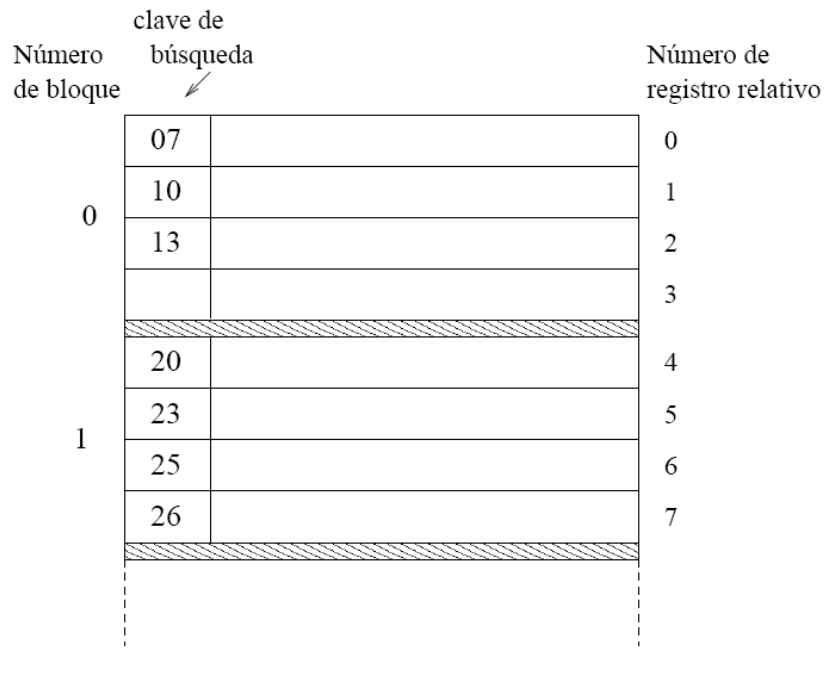
\includegraphics[scale=1,width=1\textwidth]{organizacion_secuencial.png}
\end{figure}

En cuanto a las operaciones básicas se tiene que:

\begin{itemize}
\item \textbf{Inserción de un nuevo registro}. Se busca el bloque que le corresponde, si hay sitio, se inserta, y si no hay sitio, o bien se opta por crear un nuevo bloque o bien se crea un bloque por desbordamiento. Es recomendable dejar espacio vacío en los bloques para evitar problemas de reorganización.

\item \textbf{Borrado de un registro}. Se busca el registro, y se borra, este borrado puede implicar la reorganización local de los registros de un bloque.
\end{itemize}

En resumen, ambas operaciones suponen:

\begin{itemize}
\item La escritura del bloque del registro que se inserta o borra
\item Creación o liberación de bloques de datos en el fichero secuencial
\item Creación o liberación de bloques de desbordamiento
\item Reorganización de registros entre bloques contiguos, lo que implica la escritura de los bloques implicados en el desplazamiento.
\end{itemize}

Es obvio que, esta forma de organizar los registros no está exenta de grandes inconvenientes. Estos pueden subsanarse, al menos en parte, mediante el uso de estructura adicionales que nos permitan, acelerar la localización de los datos y disminuir el número de bloques de disco transferidos. \\

Entre las técnicas más populares se encuentran:

\begin{itemize}
\item Índices
\item Acceso Directo
\end{itemize}

\textbf{Indexación.} Tiene por objeto disminiur el tiempo de acceso a los datos por una clave de búsqueda. Similar a la idea de un índice de un libro. Existen muchas forma de llevar a cabo esta idea. \\

\section{Fichero indexados}
Partimos de un fichero secuencial sobre el que disponemos una estructura adicional, el fichero índice. \\

Sus registros poseen:

\begin{itemize}
\item Campos clave (la clave de búsqueda)
\item Campo de referencia que contiene RIDs de registros.
\end{itemize}

Son más pequeños que los del fichero de datos, aunque el número de ellos es el mismo en ambos ficheros.

\begin{itemize}
\item Índice primario. La clave de búsqueda es el mismo campo clave (clave física) por el que está ordenado el fichero secuencial de datos.

\item Índice secundarios. Construidos sobre otros campos que no sean la clave físcia del fichero de datos.
\end{itemize}

\begin{figure}
\centering
\caption{Ejemplo Indexación con sólo índice primario}
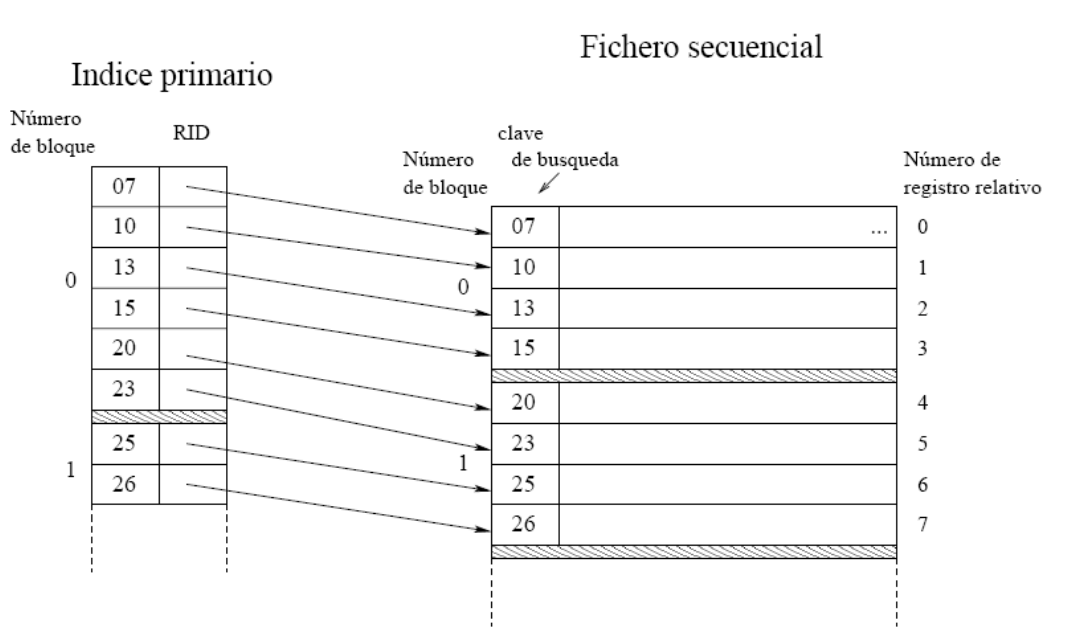
\includegraphics[scale=1,width=1\textwidth]{ejemplo_indexado.png}
\end{figure}

\textbf{Proceso de consulta}
\begin{itemize}
\item Consuslta por un valor de la clave. Sobre el índice localizamos la clave con un recorrido secuencial. Obtenemos el RID del registro requerido. Vamos a disco a recuperar el bloque de datos donde se encuentra el registro señalado por el RID. La búsqueda en el índice es más rápida.

\item Consulta por rango de valores. Búsqueda en el índie por valor de clave de la cota inferior. Recorrido de las entradas del índice que están en el intervalo, recuperando los registros correspondientes gracias a su RID.

\end{itemize}

\begin{itemize}
\item Inserción de un nuevo registro. Se realizan las mismas operaciones que en el fichero secuencial. Hay que actualizar también el índice (inserción en un fichero secuencial).

\item Borrado de un registro en el fichero de datos. Borrado de una entrada en el índice.
\end{itemize}

\textbf{Índice denso:} tienen una entrada por cada registro del fichero de datos. \\

Se puede montar un índice sobre más de un campo de un registro, es decir, la clave sería la concatenación de los campos indicados. \\

Se debe tener cuidado, un índice sobre nombre-alumno y DNI es útil para consulta que involucran, el nombre o el nombre y el DNI pero no es útil para consultas sobre el DNI. \\

\textbf{Conclusiones}. \\
Los índices aceleran el acceso a los datos, pero ralentizan las otras operaciones pues hay que mantener el índice. Por lo tanto, hay que considerar la conveniencia de crear cada índice, teniendo en cuenta la frecuencia de las consultas y la frecuencia de las operaciones de mantenimiento de los datos.

\begin{figure}[h]
\centering
\caption{Ejemplo Indexación con índice primario y secundario}
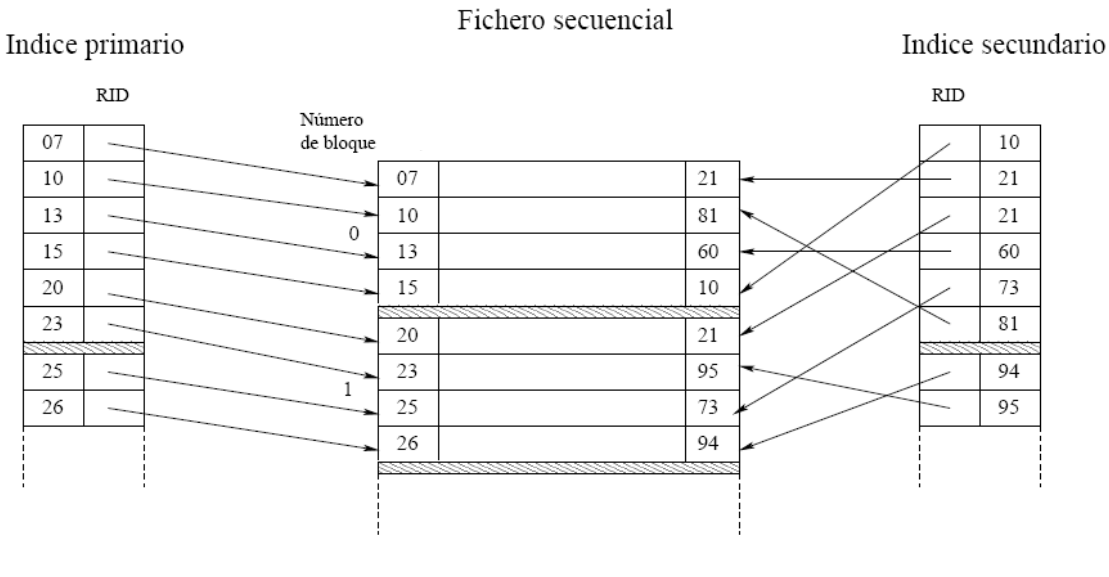
\includegraphics[scale=1,width=1\textwidth]{ejemplo_secundario.png}
\end{figure}

\textbf{Índices no densos.} \\
Lo ideal es mantener el índice en memoria principal, sin embargo, la realidad es que los índices siguen siendo muy grandes, porque contienen todos los registros del fichero que indexan. Son densos. \\

Para reducir el tamaño aparecen los índices no densos. En estos los registros se componen de la clave de búsqueda y la dirección de comienzo del bloque donde puede encontrar el registro deseado. El número de registros se reduce al número de bloques del fichero de datos. El acceso secuencial al índice no denso se acelera. \\

\textbf{Diferencias en el proceso de búsqueda.} \\

Una vez encontrado el bloque donde podría encontrar el registro, hay que cargarlo en memoria, y además hay que hacer una búsqueda secuencial. No tiene costes en términos de acceso a disco. \\

No se tiene garantía alguna de encontar el registro deseado hasta consultar el bloque de datos leído. Los índices no densos sólo se pueden definir sobre clave física. \\

Ahora bien, el mantenimiento de un índice no denso es menos costoso, puesto que la inserción y borrado de valores del índice son menos frecuentes, y sólo ocurren cuando la operación afecta al valor representativo del bloque. \\

\begin{figure}
\centering
\caption{Ejemplo índice no denso}
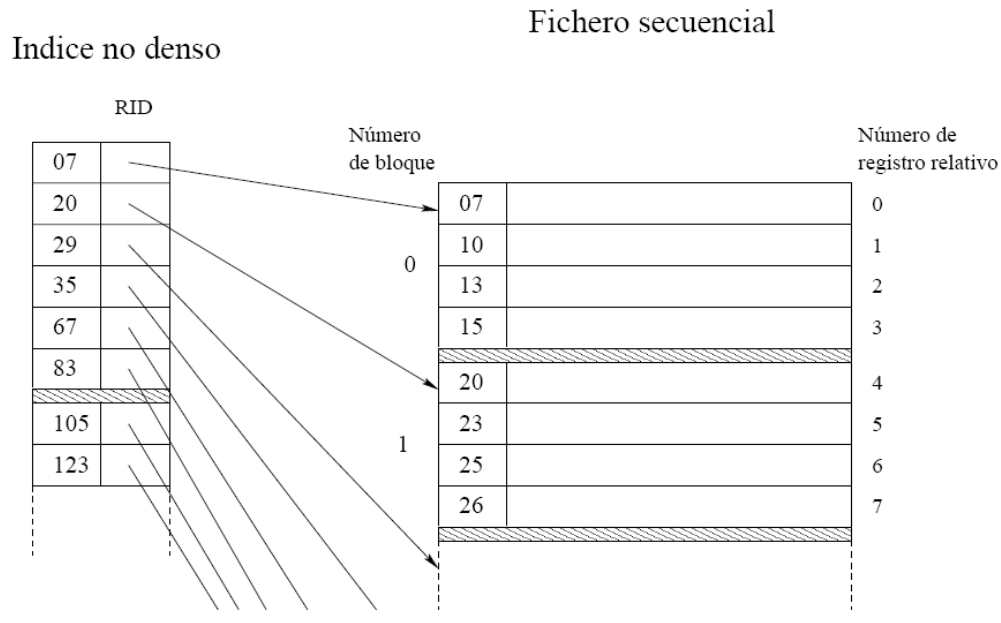
\includegraphics[scale=1,width=0.8\textwidth]{indice_no_denso.png}
\end{figure}

\textbf{Índices jerárquicos.} \\
Se vuelve al objetivo de disminuir el tiempo necesario para recorres el índice en busca de un registor. Esta vez la idea es crear índices sobre índices, con varios niveles en el acceso a los datos. \\

Un índice multinivel se compone de un índice de primer nivel sobre el fichero de datos, puede ser denso o no dependiendo de la clave, y otros índices, no densos, construidos sucesivamente unos sobre otros. \\

El tamaño de los bloques se establece con la idea de optimizar cada una de las operaciones de acceso al disco físico. Se reduce el número de accesos a disco para localizar un registro, en el peor caso se hacen tantos como niveles haya. Como consecuencia, se complica el mantenimiento del índice. \\

\begin{figure}[h]
\centering
\caption{Ejemplo Indice Jerárquico}
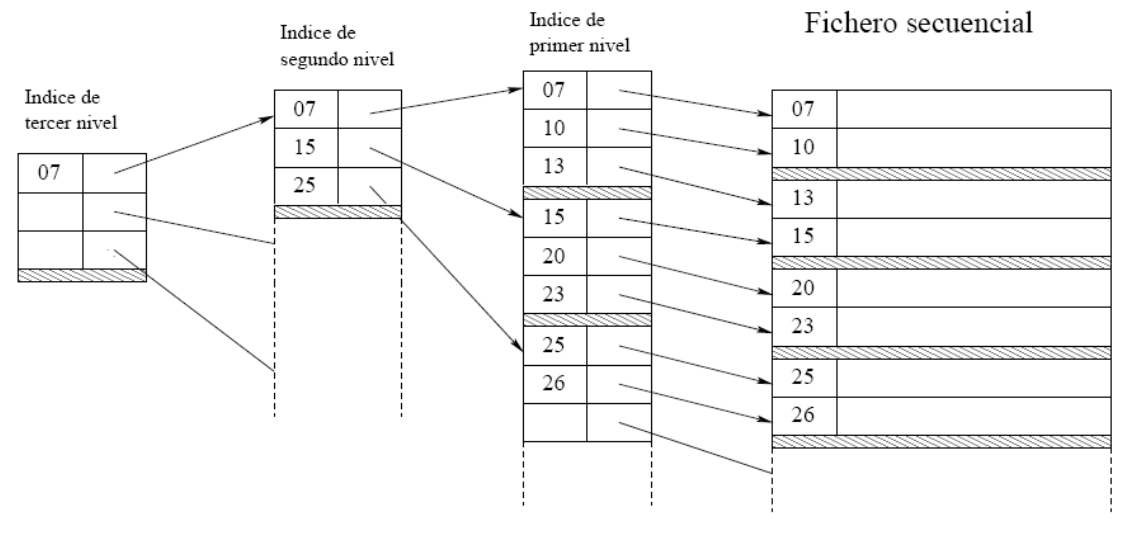
\includegraphics[scale=1,width=0.8\textwidth]{indice_jerarquico.png}
\end{figure}

\textbf{Árboles $B^+$.} \\

Estos fueron propuestos en 1972 por Bayer y McCreight son una generalización de los árboles binarios balanceados en la que los nodos pueden tener más de dos hijos. Todos los valores de la clave se encuentran alamacenados en los nodos hojas. \\

Un árbol $B^+$ de orden M (el máximo número hijos que puede tener cada nodo) es un árbol con la siguiente estructura:

\begin{itemize}
\item Nodo de nivel superior, raíz del árbol.
\item Nodos del nivel inferior, nodos hoja.
\item Cada nodo distinto de las hojas tiene como máximo M hijos.
\item Todos los nodos hoja aparecen al mismo nivel.
\item Las claves contenidas en cada nodos nos guiarán hasta el siguiente nodo del nivel inmediatamente inferior.
\item Un nodo no hoja con n hijos contiene, n-1 valores de clave almacenados, n punteros $P_i$ que apuntan a un nodo hijo.
\end{itemize}

\textbf{Restricciones dentro de los nodos:}

\begin{itemize}
\item Los valores de clave $C_i$ están ordenados dentro del nodo.
\item Los valores x del subárbol apuntado por $P_i$ cumple: $C_{i-1} \leq x < C_i$, execpto para $i=1$, donde $x < C_1$ y para $i=n$, donde $x \geq C_{n-1}$.
\end{itemize}

\textbf{Nodos hoja:}

\begin{itemize}
\item Tienen una estructura diferentes. Se componen de parejas clave-RID y punteros al siguiente nodo hoja. Algunas variantes también tiene puntero al nodo hoja anterior.
\end{itemize}

\textbf{Restricciones en nodos hojas:}

\begin{itemize}
\item Las claves aparecen ordenados en cada nodo.
\item Todas las claves han de ser menores que las del siguiente nodo en el conjunto de secuencia. 
\item Todos los nodos hoja se encuentran en el mismo nivel. Esto se debe a que es un árbol equilibrado. Además, todos los caminos desde al raíz a un nodo hoja tiene la misma longitud.
\end{itemize}

\begin{figure}
\centering
\caption{Compendio Restricciones Árboles $B^+$}
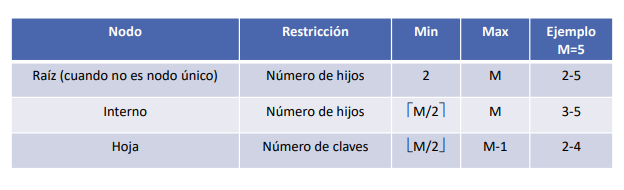
\includegraphics[scale=1,width=0.8\textwidth]{compendio_restricciones.png}
\end{figure}

\textbf{Proceso de consulta.}  \\

Para localizar un registro, navegamos desde la raíz, bajando niveles. Buscamos el registro en el nodo hoja y, en su caso, recuperamos el registro del fichero de datos gracias al RID. \\

En cuanto a las consultas por rango, se localiza el nodo hoja que contiene el valor inferior, y se recorren todos los nodos hoja hasta alcanzar el superior, recuperando los registros pertinentes del fichero de datos. \\

\textbf{Inserción y borrado:} \\

Se utilizan algoritmos que nos garantizan que el árbol resultante sea equilibrado.

\begin{figure}[h]
\centering
\caption{Ejemplo recorrido en consultas por rango de clave}
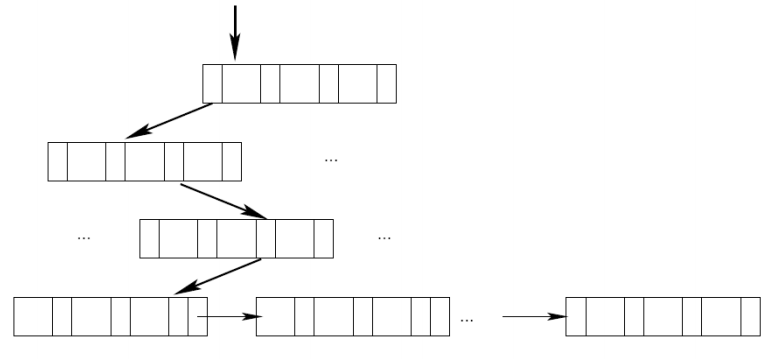
\includegraphics[scale=1,width=0.8\textwidth]{recorrido_arbol.png}
\end{figure}

\textbf{Árboles B.} \\

Los Árboles-B (B-Tree) son una variante de los $B^+$Tree en la que no se almacenan todos los valores de la clave en los nodos hoja, sino que algunos valores se van almacenando en nodos intermedios conforme se crea el árbol. \\

\textbf{Árboles $B^+$ en Bases de Datos.} \\

Son variaciones del Árbol $B^+$, de orden elevado; se procura que cada nodo tenga una capacidad de almacenamiento similar al tamaño de un bloque de datos. Esto reduce los accesos a disco que suelen ser los que determinan el rendimiento de las búsquedas en BD. 

En los nodos intermedios solo están los rangos de los valores de la clave y los punteros a los nodos hijos correspondientes. En los nodos hoja se encuentran todos los valores de la clave ordenados junto con los RIDs (rowid) que apuntan a las tuplas que contienen ese valor de la clave. \\

Los nodos hoja, que forman el conjunto secuencia, se encuentran enlazados para poder recuperar por búsquedas secuenciales, a veces se encentran doblemente enlazados, para facilitar búsquedas ascendentes y descendentes por el valor de la clave. \\

\begin{figure}[h]
\centering
\caption{Ejemplo árbol $B^+$}
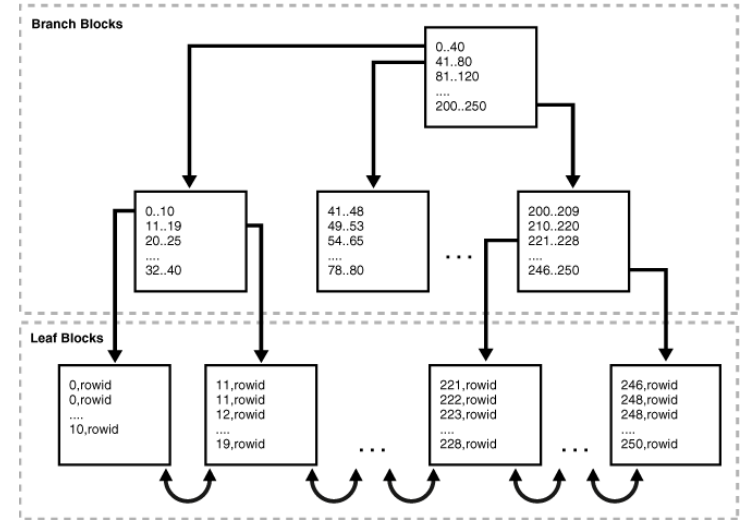
\includegraphics[scale=1,width=0.8\textwidth]{ejemplo_arbol_b+.png}
\end{figure}

\textbf{Talbas Organizadas por Índice (IOT).} Las hojas contienen las tuplas en lugar del RID. Una IOT sólo puede estar organizada de esta forma mediante una clave, aunque se pueden definir índices adicionales basados en otras claves. \\

\begin{figure}
\centering
\caption{Ejemplo IOT}
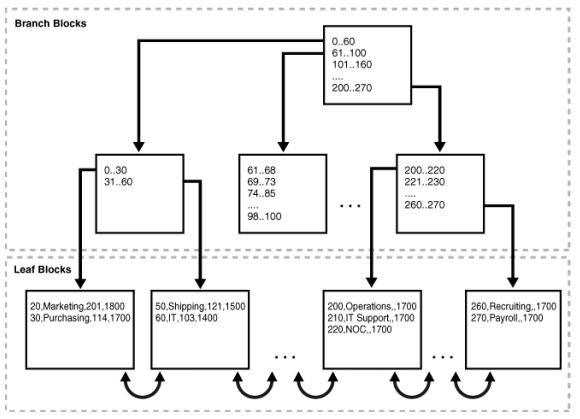
\includegraphics[scale=1,width=0.8\textwidth]{ejemplo_iot.png}
\end{figure}

\textbf{Índices clave invertida (Reverse Index).} \\

Invierte los datos del valor de la clave. Por ejemplo, para el empleado 7698 almacena 8967. \\

Este índice es adecuado para búsquedas basadas en predicados iguales. \\

Con este índice se reducen los embotellamientos (retención de bloque de BD) en el índice cuando se están introduciendo los datos de forma ascendente para los valores de la clave, puesto que todos irían a la misma entrada de índice. \\

\begin{figure}[h]
\centering
\caption{Ejemplo Índices Clave Invertida}
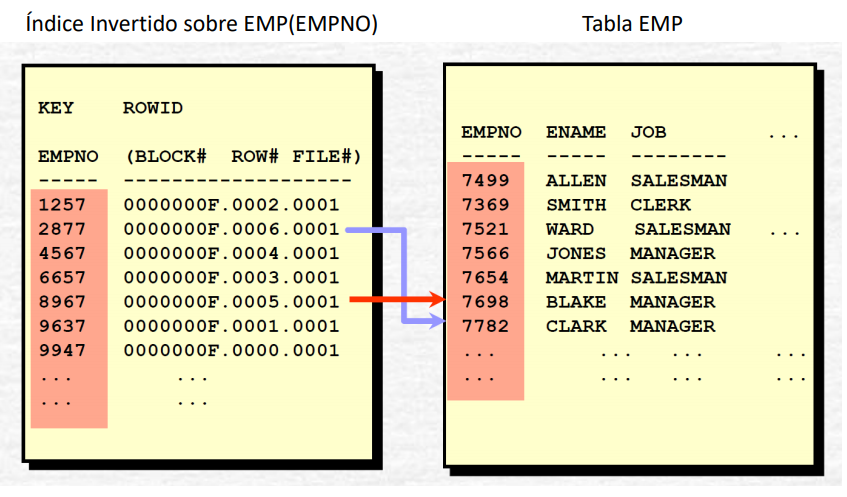
\includegraphics[scale=1,width=.8\textwidth]{tabla_emp.png}
\end{figure}

\textbf{Índices BITMAP.} \\

Para cada valor que toma la clave almacena una secuencia de bits (tantos como tuplas contenga la tabla). El bit 1 indica que ese valor está presente en la tupla, mientras que el bit 0 indica que no lo está. \\

Por una parte el B-tree es adecuado para columnas que tomen muchos valores, las actualizaciones sobre las claves no es muy costosa, sin embargo, es ineficiente para consultas usando predicados OR.\\

Por su parte el bitmap es adecuado para columnas que tomen pocos valores y es eficiente para consultas usando predicados OR, sin embargo, las actualizaciones sobre las claves son muy costosas.

\begin{figure}[h]
\centering
\caption{Ejemplo BITMAP}
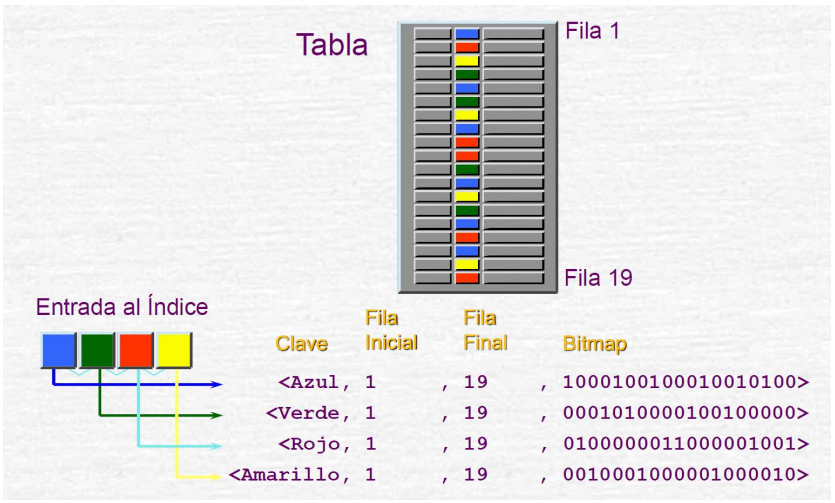
\includegraphics[scale=1,width=1\textwidth]{ejemplo_BITMAP.png}
\end{figure}

\section{Acceso Directo}
El acceso directo es otra forma de acceder a un registro almacenado. Para este tipo de acceso no hay estructura adicional, y se usa un algoritmo que nos indique directamente la posición del registro deseado. \\

\textbf{Acceso Directo.} Calcular directamente la dirección de un registro mediante la aplicación de algún algoritmo sobre un campo determinado del mismo. Este campo debe identificar unívocamente al registro. \\

\textbf{Funcionamiento.} Normalmente no es posible establecer una clave física que sea totalmente correlativa y única para cada registro. Hay que buscar un algoritmo que transforme los valores de un cierto campo en una dirección, es decir, que tome como entrada un campo clave y como salida un valor entero positivo fácilmente transformable en RID. 

\begin{figure}[h]
\centering
\caption{Ejemplo Acceso Directo}
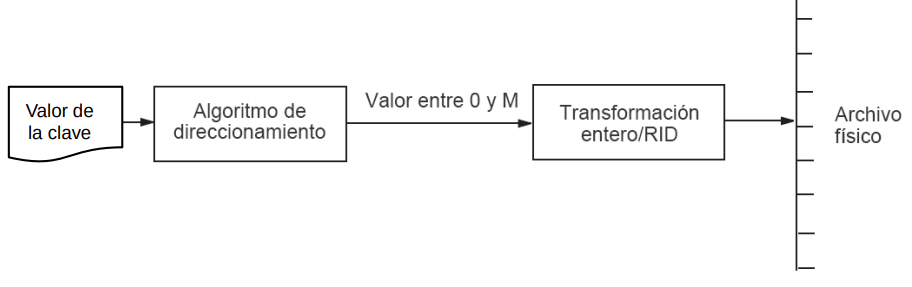
\includegraphics[scale=1,width=0.8\textwidth]{acceso_directo.png}
\end{figure}

Los algoritmos de direccionamiento no suelen mantener el orden de la clave, es decir, los registros no están almacenados según el orden de su clave física. Esto genera problema con la recuperación por intervalos. \\

Para la transformación de la clave física hay gran variedad de algoritmos, todos ellos dependiente del tipo de clave. Si la clave es alfanumérica, hay que transformarla a un valor númerico. Estos algoritmos suelen estar basado en un mecanismo de generación de número pseudoaleatorios:

\begin{itemize}
\item Cuadrados Centrales: se eleva la clave al cuadrado y se eligen tantos dígitos centrales como sea necesario.

\item Congruencias: se divide la clave por M y se toma el resto. (M suele ser primo).

\item Desplazamiento: se superponen adecuadamente los dígitos binarios de la clave y luego se suman.

\item Conversión de base: se cambia la base de numeración y se suprimen algunos dígitos resultantes.
\end{itemize}

\textbf{Problema}. Salvo que el campo se diseñe para ello, es prácticamente imposible encontrar una transformación que dé un valor entero positivo en un rango de valores limitado tal que no haya dos valores distintos de clave que den lugar al mismo número, es decir, sin que haya colisiones. \\

Los algoritmos producen huecos, esto son, zonas vacías del rango de salida, no asignadas por el algoritmo. Esto se traduce en hueco en el fichero de datos. \\

Para gestionar colisiones y huecos, lo normal es combinar el acceso directo con una gestión mediante listas de colisión:

\begin{itemize}
\item Zona de desbordamiento

\item Colisión. El registro problemático se almacena en la zona de desbordamiento. Los sinónimos (registros con claves que producen colisión) se conectan mediante una lista.
\end{itemize}

\begin{figure}[h]
\centering
\caption{Ejemplo Zona de Desbordamiento}
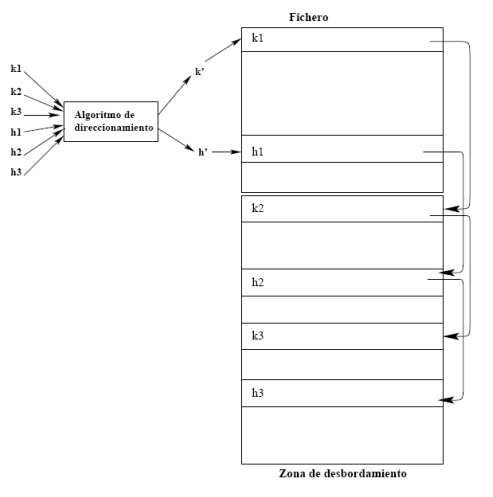
\includegraphics[scale=1,width=0.8\textwidth]{zona_desbordamiento.png}
\end{figure}

Si las listas de sinónimos crecen, entonces el acceso directo puro no resulta adecuado, pues hay que mantener las lista y la zona de desbordamiento sería casi como el fichero original. En contramedida han aparecido técnicas más sofisticadas.

\section{Hashing}

\textbf{Hashing Básico}. Si el problema principal es que los valores de las claves no están uniformemente distribuidos en el intervalo $[0,M]$, entonces se acumulan en una parte de este intervalo, por lo tanto, la solución será asignar más espacio a esa parte del intervalo. \\

La técnica sería:

\begin{itemize}
\item Se divide el espacio del fichero en 'cubos' (buckets)
\item El algoritmo de direccionamiento asigna cubos, no direcciones concretas
\item En cada 'cubo' puede haber más de un registro
\item Ciertos rangos de valores tienen asignados más cubos que otros
\item Se complementa con el uso de 'cubos de desbordamiento'.
\end{itemize}

Tendremos como parámetros:

\begin{itemize}
\item Número de cubos
\item Tamaño de los cubos (relación con bloque físicos) 'slots'
\item La transformada clave/dirección, que debe tener en cuenta la distribución de la clave según rango para que unos cubos no se llenen mucho y otros se queden muy vacíos.
\end{itemize}

Para insertar un registro, se transforma la clave, se localiza el cubo correspondiente, si hay sitio se inserta el registro y termina, y si no lo hay se sitúa el registro en un cubo de desbordamiento conectándolo con el cubo que realmente le corresponde mediante punteros. \\

Para el proceso de búsqueda se transforma la clave, se localiza el cubo correspondiente, y dentro del cubo se realiza una búsqueda secuencial, si se encuentra el registro, el proceso termina, sino se impone un barrido por punteros a través de los cubos de desbordamiento. \\

\textbf{Hashing Dinámico.} El hashing básico sigue teniendo problema, pues es necesario conocer la distribución previa de las claves para asignar adecuadamente los cubos. En otro caso siguen apareciendo huecos/colisiones. Al aumentar el número de registros, aumentan los registros en páginas de desbordamiento y se hacen necesarias las reorganizaciones. \\

\textbf{Solución:} trabajar de forma dinámica. Se parte de una configuración uniforme de pocos cubos. Los restantes, se van generando conforme se necesiten. Se asignan a los rango conforme la afluencia de registros lo demanda, por medio de hashing dinámico o extensible. \\

\textbf{Técnica:}

\begin{itemize}
\item El valor transformado del campo clave nos lleva a la entrada de una table índice que se almacena en memoria. 
\item Allí está la dirección del cubo donde se encuentran los registros que tienen asociado este valor transformado.
\item Puede ocurrir que varias entradas de la tabla conduzcan a un mismo cubo. 
\item Proceso. Inicialmetne, todas las entradas apuntan al mismo cubo. A medida que vamos insertando registros, se van generando nuevos cubos y cambiando las salidas de la tabla índice.
\end{itemize}

\textbf{Algoritmo de Hashing Dinámico}. Datos de partida:

\begin{itemize}
\item k= clave física para direccionar.
\item k'= h(k) valor entero entre 0 y M.
\item n= número de bits que tiene k' en binario.
\item d<=n, los d primero dígitos de k' seleccionan el cubo donde est'el registro y se llaman pseudo llave
\item b<d<=n, inicialmente el archivo tiene $2^b$ cubos distintos, como máximo tendrá $2^d$. Si son necesarios más, hay que aumentar d.
\end{itemize}

\begin{figure}
\centering
\caption{Ejemplo Hashing Dinámico}
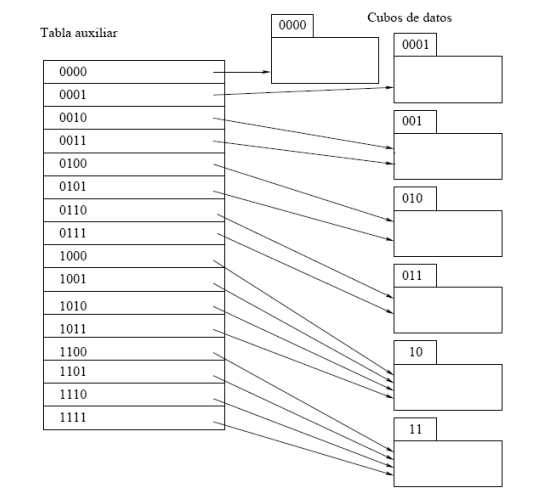
\includegraphics[scale=1,width=0.8\textwidth]{hashing_dinamico.png}
\end{figure}

Algoritmo:

\begin{itemize}
\item Se considera una tabla índice en memoria con $2^d$ filas.
\item En la primera columna de esta tabla (valores de campo clave) se sitúan todas las posibles sucesiones de d dígitos binarios, donde d es la profundidad global de la tabla.
\item Todos los cubos tiene en principio profundidad local igual a b. En principio, todas las entradas cuyos b primeros dígitos son iguales apuntan al mismo cubo. Allí se almacenan los registros cuyo valor de $k'$ tiene esos b primero dígitos. 
\item Cuando se lleva un cubo se divide en 2, poniendo en uno de ellos los registros con el dígito b+1 de $k'$ a 0 y en otro los que lo tiene igual a 1. La profundidad local de estos cubos aumenta una unidad.
\end{itemize}


El hashing dinámico supera los problemas clásicos del acceso directo. \\

Sin embargo, también tiene sus inconvenientes, pues utiliza una tabla índice adicional (nuevos accesos a disco si no cabe en memoria) y el tamaño de la table depende de 'd'.

\section{Seminario 4}
\subsection{Introducción}
Se denomina lenguaje de consulta a aquellos que permiten al usuario solicitar información de la base de datos. Normalmente, son de más alto nivel que los lenguajes de programación de propósito general, y pueden clasificarse en procedimentales y declarativos. Por ejemplo, el álgebra relacional.\\

\textbf{Procedimental.} En los lenguaje procedimentales el usuario da instrucciones al sistema para que realice una secuencia de operaciones en la BD para calcular el resultado deseado. \\

\textbf{Declarativo.} El usuario describe la información deseada sin dar un procedimiento específico para obtener esa información. Por ejemplo, el cálculo relacional (Codd, 1970). \\

\subsection{Álgebra relacional}
\textbf{Operaciones:} Las operaciones del álgebra relacional son internas dentro del conjunto de las relaciones:

\begin{itemize}
\item Entrada: una o más relaciones
\item Salida: una relación
\end{itemize}

\begin{figure}[h]
\centering
\caption{Operadores Algebra Relacional y sus notaiones}
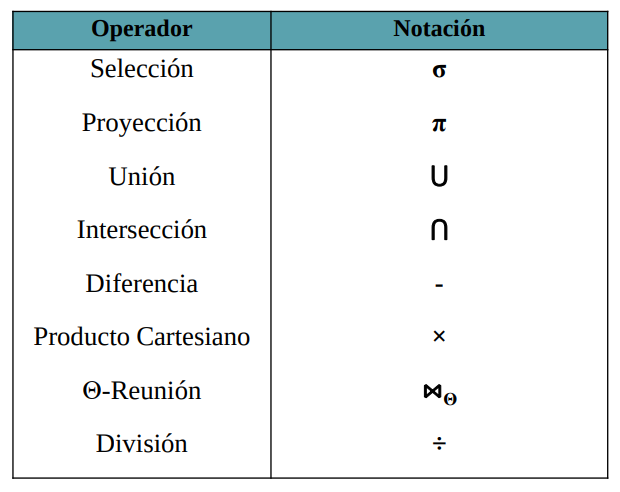
\includegraphics[scale=1,width=0.8\textwidth]{operaciones_algebra.png}
\end{figure}

Para los operadores se realida la siguiente clasificación:

\begin{itemize}
\item Con respecto al tipo de operador:
	\begin{itemize}
		\item Operadores monarios:
			\begin{itemize}
				\item Selección
				\item Proyección
			\end{itemize}
		
		\item Operadores binarios:
			\begin{itemize}
				\item Unión
				\item Intersección
				\item Diferencia
				\item Producto Cartesiano
				\item $\theta$-reunión
				\item División
			\end{itemize}
	\end{itemize}

\item Con respecto a su relación con el modelo relacional:
	\begin{itemize}
		\item Operadores de conjunto
			\begin{itemize}
				\item Unión 
				\item Diferencia
				\item Intersección
				\item Producto
			\end{itemize}
			
		\item Operadores Relacionales
			\begin{itemize}
				\item Selección
				\item Proyección
				\item $\theta$-reunión
				\item División
			\end{itemize}
	\end{itemize}

\item Con respecto a su necesidad:
	\begin{itemize}
		\item Operadores fundamentales (primitivos):
			\begin{itemize}
				\item Selección
				\item Proyección
				\item Unión
				\item Diferencia
				\item Producto Cartesiano
			\end{itemize}
		\item Operadores no fundamentales (derivados)
			\begin{itemize}
				\item Intersección
				\item $\theta$-reunión
				\item División
			\end{itemize}
	\end{itemize}
\end{itemize}

\textbf{Selección}. Sea $R[A_1,\ldots,A_n]$ una relación cualquiera, $\theta$ una propiedad asociada $\{A_1\ldots A_n\}$ y r una instancia de R. El operador $\theta$-selección aplicado a r obtiene aquellas tuplas de r para las que la propiedad $\theta$ es cierta. \textbf{Notación:} $\sigma_\theta(R)$. \\

\textbf{Proyección:}Sea $R[A_1,\ldots,A_n]$ una relación cualquiera, $\{A_i\ldots A_j\}$ un subconjunto de sus atributos y r una instancia de R. El operador proyección sobre $\{A_i\ldots A_j\}$ aplicado a R obtiene las tuplas de r eliminando de la tabla aquellos atributos no pertenecientes a $\{A_i\ldots A_j\}$ y suprimiendo las tuplas redundantes, es decir, aquellas que tras la eliminación se repitan. \textbf{Notación:} $\pi_{A_i\ldots A_j}(R)$. \\

Como una proyección produce como resultado una relación, si en el resutlado aparecen tuplas repetidas se deben descartar, esto suele ocurrir cuando, al proyectar, no se incluye una clave candidata en la lista de atributos. \\

\textbf{Composición de operadores.} El álgebra relacional se basa en la aplicación sucesiva de operadores hasta que obtenemos la tabla que contiene la solución a nuestra consulta. 

Como el resultado de una oepración es siempre una relación, dicho resultado puede usarse como operando de otra operación. \\

\textbf{Producto cartesiano.} Sea $R[A_1,\ldots,A_n]$ una relación cualquiera y r y s dos instancias de las mismas. El producto cartesiano (del álgebra) de ambas instancias es el conjunto de tuplas resultante de hacer el producto cartesiano (conjuntista) sobre los conuunto de tupls de las instancias. \textbf{Notación:} $R\times S$. \\

Propiedades del producto cartesiano:

\begin{itemize}
\item Sea $R[A_1,\ldots,A_n]$ y $S[B_1,\ldots,B_m]$ dos relaciones cualesquiera, entonces para $W[A_1\ldots A_n,B_1\ldots B_m]$ se tiene que $esquema(W)=esquema(R)\cup esquema(S).$

\item Sean $R[A_1,\ldots,A_n]$ y $S[B_1,\ldots,B_m]$ dos relaciones cualesquiera y $W=R \times S$. Sean r y s instancias de R y S respectivamente y w la correspondiente instancia de W, entonces $card(W)=card(r)\times card(s)$.
\end{itemize}

Denominación de atributos y uso de alias. Si intervienen más de una relación puede ocurrir que haya ambigüedad a la hora de referenciar atributos de las operacioens. La solución es anteponer un prefijo al nombre del atributo para indicar a la trabla a la que nos referimos. Por ejemplo $Profesor.NRP$. \\

Puede ocurrir incluso que una misma relación aparezca más de una vez en la consulta. Entonces se usa el \textbf{operador de redefinición}. Sea $R[A_1,\ldots,A_n]$ una relación cualquiera y r una instancia de R. El operador redefinición aplicado a R nos permite asignar un nuevo nombre a R. \textbf{Notación:} $\rho(R)$ = S nos permite referirnos a r como S, entonces se dice que S es un alias de R. \\

\textbf{Unión y diferencia:}

\begin{itemize}
\item \textbf{Unión.} Sean $R[A_1,\ldots,A_n]$ y $S[B_1,\ldots,B_n]$ dos relaciones tales que $\{A_1\ldots A_n\}\equiv\{B_1\ldots B_n\}$, r y s instancias de R y S, entonces el operador unión aplicado sobre R y S es el resultado de hacer la unión de r y s como conjuntos de tuplas. \textbf{Notación:} $R \cup S$. 

\item \textbf{Diferencia.} Sean $R[A_1,\ldots,A_n]$ y $S[B_1,\ldots,B_n]$ dos relaciones tales que $\{A_1\ldots A_n\}\equiv\{B_1\ldots B_n\}$, r y s  instancias de R y S, entonces el operador diferencia aplicado sobre R y S es el resultado de hacer la diferencia de r y s como conjuntos de tuplas. \textbf{Notación:} $R-S$
\end{itemize}

\textbf{$\theta$-Reunión.} Sea $R[A_1,\ldots,A_n]$ y $S[B_1,\ldots,B_m]$ dos relaciones cualesquiera, $\theta$ es una propiedad que implica a atributos de ambas relaciones, y r y s dos instancias de las mismas. Entonces la $\theta$-Reunión de R y S equivale a $\sigma_\theta(R\times S)$. \textbf{Notación:} $R \Join_\theta S$ \\

\textbf{Reunión Natural}. Sea $R[A_1,\ldots,A_n]$ y $S[B_1,\ldots,B_m]$ dos relaciones tales que existen $\{A_i\ldots A_j\} \subseteq \{A_1\ldots A_n\}$ y $\{B_i\ldots B_j\}\subseteq \{B_1\ldots B_m\}$ tales que $\forall k \in \{i\ldots j\}$, $A_k = B_k$, r y s son dos instancias de las mismas. Entonces, la reunión natural de R y S equivale a $\pi_{(\{A_1\ldots A_n\}\cup\{B_1\ldots B_m\})-\{A_i\ldots A_j\}}(\sigma_{(r.A_i=s.B_i)\land\ldots\land(r.A_j=s.B_j)}(R\times S))$. \textbf{Notación:} $R\Join S$. \\

\textbf{Intersección.} Sean $R[A_1,\ldots,A_n]$ y $S[B_1,\ldots,B_n]$ dos relaciones tales que $\{A_1\ldots A_n\}\equiv\{B_1\ldots B_n\}$, r y s  instancias de R y S, entonces el operador instersección aplicado sobre R y S es el resutlado de hacer la instersección r y s como conjunto de tuplas. \textbf{Notación:} $R \cap S$. \\

Propieades:
\begin{itemize}
\item Sean R y S relaciones cualquiera y r y s dos instancias de las mismas, se verifica que $R \cap S=R-(R-S)$
\end{itemize}

\textbf{División:} Sean $R[A_1,\ldots,A_n]$ y $S[B_1,\ldots,B_n]$ y las instanias r y s. La divisón de R con respecto a S es la instancia w de una relación $W[A_1\ldots A_n]$, que verifica:

\begin{itemize}
\item $\forall u \in w$; $\forall v \in s$, $\exists t \in r|t[A_1\ldots A_n]=u,\> t[B_1\ldots B_n]=v$
\end{itemize}

\textbf{Notación:} $R \div S$ 

Propiead:

\begin{itemize}
\item Sean $R[A_1,\ldots,A_n]$ y $S[B_1,\ldots,B_n]$ y las instanias r y s, entonces $R \div S=\pi_{A_1\ldots A_n}(S)-\pi_{A_1\ldots A_n}((\pi_{A_1\ldots A_n}(R)\times S)-R)$, es decir, toda división se puede escribir en función de proyecciones y selecciones.
\end{itemize}

\textbf{Eficiencia de las consultas:} con álgebra relacional a cada expresión le corresponde una única tabla. Cada consulta puede resolverse con más de una expresión, luego hay que elegir en términos de eficiencia. En un SGBD hay un componente que se encarga de paliar los efectos de un mal usuario, un optimizador de consultas. Este tiene algunas reglas básicas, por ejemplo, las selecciones limitan cuanto antes el número de tuplas, y análogo para las proyecciones. 

Normalmente los SGBDs no publican sus estrategias de optimización, pues es una ventaja competitiva. \\

\subsection{Otros lenguajes de consultas formales}
\textbf{Lenguaje procedimental.} El usuario da instrucciones al sistema para que realice una secuencia de operaciones en la BD para calcular el resutlado deseado. \\

\textbf{Lenguaje declarativo.} El usuario describe el resultado sin dar un procedimiento específico para obtener esa información \\

\textbf{Cálculo de predicados.} Se ha adacptado el cálculo de predicados para crear un lenguaje para bases de datos relacionales. Dos formas:

\begin{itemize}
\item Cálculo relacional orientado a tuplas (CRT), que emplea variables de tupla que toman valores en tuplas de las relaciones de nuestra BD. 

\item Cálculo relacional orientado a dominios (CRD), que utiliza variables de dominio, que toman valores de los dominios asociados a los atributos de las realciones de nuestra BD.
\end{itemize}

\subsection{Relación de Álgebra Relacional}
\begin{figure}[h]
\centering
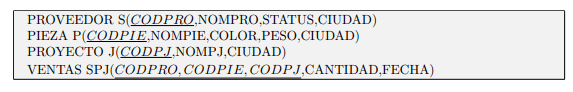
\includegraphics[scale=1,width=1\textwidth]{ejer1.png}
\end{figure}
\textbf{a) Encontrar los códigos de los proveedores que suministran alguna pieza a J1.}

\begin{equation*}
\pi_{codpro}(\sigma_{codpj=J1}(VENTAS))
\end{equation*}

\textbf{b) Encontrar los suministros cuya cantidad supere las 100 unidades.}

\begin{equation*}
\sigma_{cantidad>100}(VENTAS)
\end{equation*}

\textbf{c) Encontrar los nombres de proveedores, piezas y proyectos que se encuentren en
la misma ciudad.}


Esta respuesta se puede mejorar haciendo antes del producto cartesiano las correspondientes proyecciones.´
\begin{equation*}
\pi_{nompro,codpie,codpj}(\sigma_{J.ciudad=P.ciudad \> AND \> J.ciudad=S.ciudad}(J\times P\times S))
\end{equation*}

Como el único atributo en común de las tablas de proveedor, pieza y proyecto es la ciudad, si se reune naturalente estas tres se hace en función de la ciudad.
\begin{equation*}
\pi_{nompro,codpie,codpj}(J\Join P \Join S)
\end{equation*}

\textbf{d) Encontrar los nombres de las piezas suministradas por los proveedores de Londres.}
\begin{equation*}
\pi_{SPJ.nompie}(\sigma_{SPJ.codpro=S.codpro \> AND  \> S.ciudad=Londres}(SPJ \times S)) 
\end{equation*}


Como la tabla de proveedores y la de ventas únicamente comparten el codigo del proveedor se reunen naturalmente por este atributo, luego se puede quitar una de las condiciones en la selección.
\begin{equation*}
\pi_{nompie}(\sigma_{ciudad=Londres}(SPJ \Join S))
\end{equation*}

\textbf{e) Encontrar todas las parejas de ciudades tales que la primera sea la de un proveedor y la segunda la de un proyecto entre los cuales haya algún suministro.}

\begin{equation*}
\pi_{S.ciudad,J.ciudad}(\sigma_{SPJ.codpro=S.codpro \> AND \> SPJ.codpj=J.codpj}(SPJ\times J \times S))
\end{equation*}

\textbf{f ) Encontrar los códigos de las piezas suministradas a algún proyecto por un proveedor que se encuentre en la misma ciudad que el proyecto.}

\begin{equation*}
\pi_{codpie}(\sigma_{SPJ.codpro=S.codpro \> AND \> SPJ.codpj=J.codpj \> AND \> S.ciudad=J.ciudad}(SPJ\times J\times S))
\end{equation*}

\begin{equation*}
\pi_{codpie}(J \Join (SPJ \Join S))
\end{equation*}

\textbf{g) Encontrar los códigos de los proyectos que tienen al menos un proveedor que
no se encuentre en su misma ciudad.}

\begin{equation*}
\pi_{J.codpj}(\sigma_{SPJ.codpro=S.codpro \> AND \> SPJ.codpj=J.codpj \> AND \> S.ciudad<>J.ciudad}(SPJ\times J\times S))
\end{equation*}

\begin{equation*}
\pi_{codpj}(\sigma_{J.codpj=SPJ.codpj \> AND \> S.ciudad<>J.ciudad}((SPJ \Join S)\times J))
\end{equation*}

\textbf{h) Mostrar todas las ciudades de donde proceden piezas y las ciudades donde hay
proyectos.}

El enunciado es ambiguo, esta solución considera el conjunto formado por todas las ciudades de las cuales procede una pieza o hay un proyecto
\begin{equation*}
\pi_{ciudad}(P)\cup\pi_{ciudad}(J)
\end{equation*}

En esta solución se muestran las ciudades donde proceden piezas y además son ciudad de algún proyecto
\begin{equation*}
\pi_{ciudad}(P)\cap\pi_{ciudad}(J)
\end{equation*}

\textbf{i) Mostrar todas las ciudades de los proveedores en las que no fabriquen piezas.}

En esta solución a las ciudades de los proveedores se les quitan las ciudades donde se fabrican piezas, quedando así las ciudades donde no se fabrican piezas
\begin{equation*}
\pi_{ciudad}(S)-\pi_{ciudad}(P)
\end{equation*}

\textbf{j) Mostrar todas las ciudades de los proveedores en las que además se fabriquen
piezas.}

En esta solución al conjunto de las ciudades de los proveedores se le intersecan el conjunto de las ciudades donde se fabrican piezas, quedando las ciudades con ambas condiciones.
\begin{equation*}
\pi_{ciudad}(S)\cap\pi_{ciudad}(P)
\end{equation*}

\textbf{k) Encontrar los códigos de los proyectos que usan una pieza que vende S1.}

\begin{equation*}
\pi_{codpj}(SPJ\Join(\pi_{codpie}(\sigma_{codpro=S1}(SPJ))))
\end{equation*}

\textbf{l) Encontrar la cantidad más pequeña enviada en algún suministro.}

\begin{equation*}
\rho(SPJ)=venta
\end{equation*}

\begin{equation*}
\pi_{cantidad}(SPJ) -
\end{equation*}

\begin{equation*}
\pi_{venta.cantidad}(\sigma_{SPJ.cantidad < venta.cantidad}(\pi_{cantidad}(venta)\times \pi_{cantidad}(SPJ)))
\end{equation*}

\textbf{m) Encontrar los códigos de los proyectos que no utilizan una pieza roja suministrada por un proveedor de Londres.}

\begin{equation*}
\pi_{codpj}(J)-\pi_{codpj}(\sigma_{ciudad=Londres \> AND \> color=rojo}(SPJ\Join(\sigma_{codpie,color}(P))\Join(\sigma_{codpro,ciudad}(S))))
\end{equation*}

\textbf{n) Encontrar los códigos de los proyectos que tienen como único proveedor a S1.}

\begin{equation*}
\pi_{codpj}(SPJ)-\pi_{codpj}(\sigma_{codpro<>S1}(SPJ)))
\end{equation*}

\textbf{ñ) Encontrar los códigos de las piezas que se suministran a todos los proyectos de
París.}

\begin{equation*}
\pi_{codpie,codpj}(SPJ) \div \pi_{codpj}(\sigma_{ciudad=Paris}(J))
\end{equation*}

\textbf{o) Encontrar los códigos de los proveedores que venden la misma pieza a todos los
proyectos.}

\begin{equation*}
\pi_{codpro}((\pi_{codpro,codpie,codpj}(SPJ))\div \pi_{codpj}(J))
\end{equation*}

\textbf{p) Encontrar los códigos de los proyectos a los que S1 suministra todas las piezas
existentes.}

\begin{equation*}
\pi_{codpj,codpie}(\sigma_{codpro=S1}(SPJ)) \div \pi_{codpie}(P)
\end{equation*}

\textbf{q) Mostrar los códigos de los proveedores que suministran todas las piezas a todos
los proyectos.}

\begin{equation*}
	(\pi_{codpro,codpie,codpj}(SPJ) \div \pi_{codpj}(J)) \div \pi_{codpie}(P)
\end{equation*}

\begin{figure}[h]
\centering
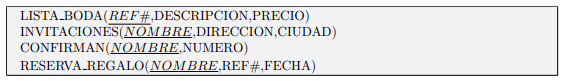
\includegraphics[scale=1,width=1\textwidth]{ejer_2.png}
\end{figure}

\textbf{a) Encontrar los regalos (descripción) que no han sido reservados.}

\begin{equation*}
\pi_{descripcion}(\pi_{ref,descripcion}(LISTA)-\pi_{ref,descripcion}(RESERVA\Join LISTA))
\end{equation*}

\begin{equation*}
\pi_{descripcion}(LISTA \Join (\pi_{ref}(LISTA)-\pi_{ref}(RESERVA)))
\end{equation*}

\textbf{b) Encontrar la dirección de los invitados que confirman la asistencia de más de
dos personas.}

\begin{equation*}
\pi_{direccion}(\sigma_{numero>2}(INVITACIONES \Join CONFIRMAN))
\end{equation*}

\textbf{c) Encontrar el nombre y la referencia del regalo más caro ya reservado.}

\begin{equation*}
\rho(LISTA\Join RESERVA)=A
\end{equation*}

\begin{equation*}
\pi_{nombre,ref}(RESERVA)-\pi_{nombre,ref}(\sigma_{A_2.precio>A_1.precio}(A_1\times A_2))
\end{equation*}

\begin{figure}[h]
\centering
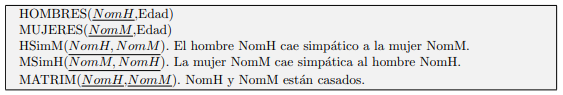
\includegraphics[scale=1,width=1\textwidth]{ejer3.png}
\end{figure}

\textbf{a) Hallar las parejas de hombres y mujeres que se caen mutuamente simpáticos,
con edades entre 20 y 30 años y que no estén casados entre sí.}

\begin{equation*}
\rho(\sigma_{edad<=30 \> AND \> edad>=30}(HOMBRES))=A
\end{equation*}

\begin{equation*}
\rho((HSimM \Join MSimH))=B
\end{equation*}

\begin{equation*}
\rho(\sigma_{edad<=30 \> AND \> edad>=30}(MUJERES))=C
\end{equation*}

\begin{equation*}
\pi_{NomH,NomM}(A\Join B\Join C)-MATRIM
\end{equation*}

\textbf{b) Hallar las mujeres casadas a las que no cae simpático su marido.}

\begin{equation*}
\pi_{NomM}(MATRIM-(MATRIM\cap \pi_{NomH,NomM}(HSimM)))
\end{equation*}

\textbf{c) Hallar los hombres a lo que no les cae simpática ninguna mujer.}

\begin{equation*}
\pi_{NomH}(HOMBRES)-\pi_{NomH}(MSimH)
\end{equation*}

\textbf{d) Hallar las mujeres casadas a las que no les cae simpático ningún hombre casado.}

\begin{equation*}
\pi_{NomM}(MATRIM)=A
\end{equation*}

\begin{equation*}
\pi_{NomH}(MATRIM)=B
\end{equation*}

\begin{equation*}
A-\pi_{NomM}(A\Join (B\Join HSimM))
\end{equation*}

\begin{figure}[h]
\centering
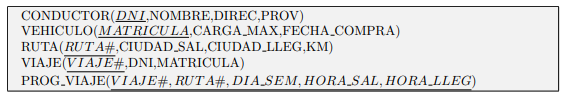
\includegraphics[scale=1,width=1\textwidth]{ejer4.png}
\end{figure}

\textbf{a) Encontrar entre qué dos ciudades se realiza el viaje más largo.}

\begin{equation*}
\pi_{sal,lleg}(R)-\pi_{R_1.sal,R_1.lleg}(\sigma_{R_1.KM<R_2.KM}(R_1\times R_2))
\end{equation*}

\textbf{b) Listar los nombres de los conductores que hayan llevado todos los camiones de
la empresa.}

\begin{equation*}
\pi_{nombre,matric}(C\Join Viaje)\div \pi_{matric}(Veh)
\end{equation*}

\textbf{c) Encontrar qué días de la semana se hacen viajes entre Granada y Sevilla por
la mañana (antes de las 13h.)}

\begin{equation*}
\theta=(CS=Sevilla \> AND \> CLL=Granada) \> OR \> (CS=Granada \>AND \>CLL=Sevilla)
\end{equation*}

\begin{equation*}
\gamma=SAL<13 
\end{equation*}

\begin{equation*}
\pi_{dia\_sem}(\sigma_{\gamma \> AND \> \theta}(PROG_VIAJE\Join VIAJE))
\end{equation*}

\textbf{d) Encontrar las rutas que se hacen todos los días de la semana, suponiendo que
hay viajes todos los días.}

\begin{equation*}
\pi_{ruta,dia\_sem}(PROG) \div \pi_{dia\_sem}(PROG)
\end{equation*}

\begin{figure}[h]
\centering
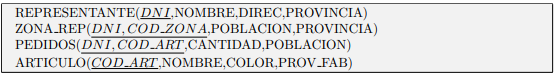
\includegraphics[scale=1,width=1\textwidth]{ejer5.png}
\end{figure}

\textbf{a) Listar las provincias que son visitadas por todos los representantes.}

\begin{equation*}
\pi_{prov,DNI}(ZONA)\div \pi_{DNI}(REP)
\end{equation*}

\textbf{b) Encontrar los representantes que venden fuera de su provincia artículos fabricados en su provincia.}(Aportación de Carlos Romero Cruz)

\begin{equation*}
\pi_{DNI}(\sigma_{R.provincia\neq ZR.provincia}(R\Join ZR)\Join \sigma_{prov\_fab=R.provincia}(P\Join A))
\end{equation*}

\begin{equation*}
\pi_{DNI}(\sigma_{A.prov<> B.prov\_f}(A\Join B))
\end{equation*}

\textbf{d) Mostrar las zonas que incluyen a una sola población.}
\begin{equation*}
\rho(\pi_{cod\_zona,poblacion}(zona_rep))=A
\end{equation*}

\begin{equation*}
\theta=(A_1.cod\_zona=A_2.cod\_zona \> AND \> A_1.pob<>A_2.pob)
\end{equation*}

\begin{equation*}
\pi_{A.cod\_zona}(A)-\pi_{A_1.cod\_zona}(\sigma_{\theta}(A_1\times A_2))
\end{equation*}
\textbf{e) Encontrar el código del artículo vendido en mayor cantidad.}

\begin{equation*}
\rho(\pi_{cod\_art,cantidad}(pedidos))=A
\end{equation*}

\begin{equation*}
\pi_{cod\_art}(A)-\pi_{A_1.cod\_art}(\sigma_{A_1.cantidad < A_2.cantidad}(A_1\times A_2))
\end{equation*}

\begin{figure}[h]
\centering
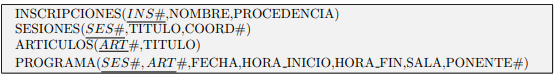
\includegraphics[scale=1,width=1\textwidth]{ejer6.png}
\end{figure}

\textbf{a) Mostrar los nombres de los ponentes que coordinan su propia sesión.}

\begin{equation*}
\pi_{nombre}(\sigma_{ins=ponente \> OR \> ins=coord}((\sigma_{ponente=coord}(SES\Join PROG))\times INS))
\end{equation*}

\textbf{b) Seleccionar los coordinadores que coordinan una única sesión.}

\begin{equation*}
\rho(\pi_{ses,coord}(sesiones))=A
\end{equation*}

\begin{equation*}
\pi_{coord}(A)-\pi_{A_1.coord}(\sigma_{A_1.coord=A_2.coord\> AND \> A_1.ses<>A_2.ses}(A_1\times A_2))
\end{equation*}

\textbf{c) Mostrar el título de los artículos que se exponen en primer y último lugar.}

\begin{equation}
\rho(S\Join P)=A
\end{equation}

\begin{equation*}
\rho(\pi_{titulo}(A)-\pi_{A_1.titulo}(\sigma_{A_1.HI>A_2.HI}(A_1\times A_2)))=C
\end{equation*}

\begin{equation*}
\rho(\pi_{titulo}(A)-\pi_{A_1.titulo}(\sigma_{A_1.HI<A_2.HI}(A_1\times A_2)))=D
\end{equation*}

\begin{equation*}
C\cup D
\end{equation*}



\end{document}
